%\documentclass[fleqn]{article}
\documentclass[nocopyrightspace,natbib]{sigplanconf}
%\documentclass[nocopyrightspace]{sigplanconf}

\usepackage{xspace,pads,amsmath,math-cmds,
            math-envs,inference-rules,times,
            verbatim,alltt,multicol,proof,url}
\usepackage{epsfig}
\usepackage{code} 
%\setlength{\oddsidemargin}{0in}
%\setlength{\evensidemargin}{0in}
%\setlength{\textwidth}{6.5in}
%\setlength{\textheight}{8.5in}

\begin{document}

\conferenceinfo{PLDI'11,}{} 
\copyrightyear{2011} 
\copyrightdata{} 

\title{Forest: A Language and Toolkit For Programming with File System Fragments}

\authorinfo{Kathleen Fisher}
	   {AT\&T Labs Research}
           {\mono{kfisher@research.att.com}}
\authorinfo{Nate Foster}
           {Cornell University}
           {\mono{jnfoster@cs.cornell.edu}}
\authorinfo{David Walker}
           {Princeton University}
           {\mono{{dpw}@CS.Princeton.EDU}}

\newcommand{\cut}[1]{}
\newcommand{\reminder}[1]{{\it #1 }}
\newcommand{\edcom}[1]{\textbf{{#1}}}
\newcommand{\poplversion}[1]{#1}
\newcommand{\trversion}[1]{}

\newcommand{\appref}[1]{Appendix~\ref{#1}}
\newcommand{\secref}[1]{Section~\ref{#1}}
\newcommand{\tblref}[1]{Table~\ref{#1}}
\newcommand{\figref}[1]{Figure~\ref{#1}}
\newcommand{\listingref}[1]{Listing~\ref{#1}}
%\newcommand{\pref}[1]{{page~\pageref{#1}}}

\newcommand{\eg}{{\em e.g.}}
\newcommand{\cf}{{\em cf.}}
\newcommand{\ie}{{\em i.e.}}
\newcommand{\etal}{{\em et al}}
\newcommand{\etc}{{\em etc.\/}}
\newcommand{\naive}{na\"{\i}ve}
\newcommand{\role}{r\^{o}le}
\newcommand{\forte}{{fort\'{e}\/}}
\newcommand{\appr}{\~{}}

\newcommand{\bftt}[1]{{\ttfamily\bfseries{}#1}}
\newcommand{\kw}[1]{\bftt{#1}}
\newcommand{\pads}{\textsc{pads}}
\newcommand{\padsc}{\textsc{pads/c}}
\newcommand{\padx}{\textsc{padx}}
\newcommand{\ipads}{\textsc{ipads}}
\newcommand{\ir}{\textsc{IR}}
\newcommand{\padsl}{\textsc{padsl}}
\newcommand{\padsml}{\textsc{pads/ml}}
%\newcommand{\padsd}{\textsc{pads/d}}
\newcommand{\learnpads}{{\textsc{learnpads}}}
\newcommand{\padsd}{\textsc{Gloves}}
\newcommand{\blt}{\textsc{blt}}
\newcommand{\ddc}{\textsc{ddc}}
\newcommand{\ddl}{\textsc{ddl}}
\newcommand{\C}{\textsc{C}}
\newcommand{\perl}{\textsc{Perl}}
\newcommand{\ml}{\textsc{ml}}
\newcommand{\smlnj}{\textsc{sml/nj}}
\newcommand{\ocaml}{\textsc{OCaml}\xspace}
\newcommand{\haskell}{\textsc{haskell}\xspace}
\newcommand{\ocamlbig}{\textsc{OCAML}\xspace}
\newcommand{\java}{\textsc{java}}
\newcommand{\xml}{\textsc{xml}}
\newcommand{\html}{\textsc{html}}
\newcommand{\xpath}{\textsc{xpath}}
\newcommand{\xquery}{\textsc{xquery}}
\newcommand{\datascript}{\textsc{datascript}}
\newcommand{\packettypes}{\textsc{packettypes}}
\newcommand{\erlang}{\textsc{Erlang}}
\newcommand{\camlp}{\cd{Camlp4}}
\newcommand{\ocamlnet}{\cd{Ocamlnet} \cd{2}}

\newcommand{\totalcost}[2]{\textsc{Cost}(#1,#2)}
\newcommand{\costdescription}[1]{\textsc{CT}(#1)}
\newcommand{\normcostdescription}{\textsc{NCT}}
\newcommand{\costdata}[2]{\textsc{CD}(#2 \; | \; #1)}
\newcommand{\acostdata}[2]{\textsc{ACD}(#2 \; | \; #1)}
\newcommand{\adc}[2]{\textsc{CD'}(#2 \; | \; #1)}
\newcommand{\cardt}{\textsc{Card}}
\newcommand{\costvar}[1]{\textsc{CV}(#1)}
\newcommand{\costchar}[1]{\textsc{CA}(#1)}
\newcommand{\coststring}[1]{\textsc{CS}(#1)}
\newcommand{\costint}[1]{\textsc{CI}(#1)}
\newcommand{\costparam}[1]{\textsc{CP}(#1)}
\newcommand{\costconst}[1]{\textsc{CC}(#1)}

\newcommand{\dibbler}{Sirius}
\newcommand{\ningaui}{Altair}
\newcommand{\darkstar}{Regulus}

\newcommand{\vizGems}{Arrakis}

\newcommand{\comon}{CoMon\xspace}
\newcommand{\planetlab}{PlanetLab\xspace}
\newcommand{\monall}{Monall\xspace}
%% \newcommand{}{}


%% \newcommand{\IParray}[4]{{\tt Parray} \; #1 \; \[#2, #3, #4\]}

\newcommand{\figHeight}[4]{\begin{figure}[tb]
	\centerline{
	            \epsfig{file=#1,height=#4}}
	\caption{#2}
	\label{#3}
	\end{figure}}

\newcommand{\myalt}{\ensuremath{\; | \;}}
\newcommand{\normal}[1]{\ensuremath{\bar{#1}}}
\newcommand{\relativee}[2]{\ensuremath{{\cal R}(#1 \; || \; #2)}}
\newcommand{\srelativee}[2]{\ensuremath{{\cal S}(#1 \; || \; #2)}}
\newcommand{\addh}[2]{\ensuremath{#1 \oplus #2}}

\newcommand{\irstruct}[1]{{\tt struct}\{#1\}}
\newcommand{\irunion}[1]{{\tt union}\{#1\}}
\newcommand{\irenum}[1]{{\tt enum}\{#1\}}
\newcommand{\irarray}[1]{{\tt array}\{#1\}}
\newcommand{\irarrayFW}[2]{{\tt arrayFW}\{#1\}[#2]}
\newcommand{\irswitch}[2]{{\tt switch}(#1)\{#2\}}
\newcommand{\iroption}[1]{{\tt option}\{#1\}}
\newcommand{\setof}[1]{\lsem #1 \rsem}
\newcommand{\goto}{\Rightarrow}
\newcommand{\Pvoid}{{\tt Pvoid}}
\newcommand{\Pempty}{{\tt Pempty}}
\newcommand{\sskip}{\hspace*{5mm}}
\newcommand{\shrink}{\vspace*{-4mm}}

% Semantics
\newcommand{\setalt}{{\; | \;}}
\newcommand{\denote}[1]{\lsem #1 \rsem}
\newcommand{\lsem}{{[\![}}
\newcommand{\rsem}{{]\!]}}
\newcommand{\turn}{\vdash}
\newcommand{\meta}{m}
\newcommand{\nested}{n}
\newcommand{\mytime}[1]{#1.t}
\newcommand{\myds}[1]{#1.ds}
\newcommand{\myval}[1]{#1.nest}
\newcommand{\generatedloc}{\ensuremath{\mathtt{nowhere}}}
\newcommand{\environment}{E}
\newcommand{\universe}{U}
\newcommand{\selectOne}{\ensuremath{\mathsf{earliest}}}
% core feed semantics
\newcommand{\csemantics}[3]{{\cal C}\lsem #1 \rsem_{{#2} \, {#3}}}
% feed semantics
\newcommand{\semantics}[3]{{\cal F}\lsem #1 \rsem_{{#2} \, {#3}}}
% expression semantics
\newcommand{\esemantics}[2]{{\cal E}\lsem #1 \rsem_{{#2}}}
%\newcommand{\esemantics}[2]{#2(#1)}

% Host language types
\newcommand{\ty}{\ensuremath{\tau}}
\newcommand{\basety}{\ensuremath{b}}
\newcommand{\arrow}{\rightarrow}
\newcommand{\optionty}[1]{\ensuremath{#1 \; \mathsf{option}}}
\newcommand{\listty}[1]{\ensuremath{#1 \; \mathsf{list}}}
\newcommand{\setty}[1]{\ensuremath{#1 \; \mathsf{set}}}
\newcommand{\feedty}[1]{\ensuremath{#1 \; \mathsf{feed}}}
\newcommand{\corety}[1]{\ensuremath{#1 \; \mathsf{core}}}
\newcommand{\schedulety}{\ensuremath{\mathsf{sched}}}
\newcommand{\timety}{\ensuremath{\mathsf{time}}}
\newcommand{\locty}{\ensuremath{\mathsf{loc}}}
\newcommand{\boolty}{\ensuremath{\mathsf{bool}}}
\newcommand{\unitty}{\ensuremath{\mathsf{unit}}}
\newcommand{\stringty}{\ensuremath{\mathsf{string}}}
\newcommand{\metatype}[1]{\ensuremath{\mathsf{meta}(#1)}}
\newcommand{\nestedtype}[1]{\ensuremath{\mathsf{nest}(#1)}}
\newcommand{\dsty}{\ensuremath{\mathsf{ds}}}

\newcommand{\dom}{\ensuremath{\mathsf{dom}}}
\newcommand{\ueq}[3]{\ensuremath{#1 =_{#2} #3}}
\newcommand{\fsubset}[3]{\ensuremath{#1 \subseteq_{#2} #3}}
\newcommand{\feq}[3]{\ensuremath{#1 =_{#2} #3}}

% Expressions
\newcommand{\expression}{e}
\newcommand{\constant}{c}
\newcommand{\ds}{\ensuremath{ds}}
\newcommand{\boolf}{\ensuremath{\mathtt{false}}}
\newcommand{\boolt}{\ensuremath{\mathtt{true}}}
\newcommand{\loc}{\ensuremath{\ell}}
\newcommand{\feed}{\ensuremath{F}}
\newcommand{\corefeed}{\ensuremath{C}}
\newcommand{\generalvar}{\ensuremath{x}}
\newcommand{\feedvar}{\ensuremath{x}}
\newcommand{\itemvar}{\ensuremath{x}}
\newcommand{\data}{\ensuremath{v}}
\newcommand{\atime}{\ensuremath{t}}
\newcommand{\astring}{\ensuremath{w}}
\newcommand{\unit}{\ensuremath{()}}
\newcommand{\schedule}{\ensuremath{s}}
\newcommand{\parser}{\ensuremath{p}}
\newcommand{\none}{\ensuremath{\mathtt{None}}}
\newcommand{\some}[1]{\ensuremath{\mathtt{Some}\; #1}}
\newcommand{\inl}[1]{\ensuremath{\mathtt{inl}\; #1}}
\newcommand{\inr}[1]{\ensuremath{\mathtt{inr}\; #1}}
\newcommand{\casedata}[2]{{\tt switch}(#1)\{#2\}}
%\newcommand{\nillist}{\ensuremath{\mathtt{nil}}}
\newcommand{\nillist}{\ensuremath{[\,]}}
%\newcommand{\conslist}[2]{\ensuremath{\mathtt{cons} (#1,#2)}}
\newcommand{\conslist}[2]{\ensuremath{[#1,\ldots,#2]}}
\newcommand{\nilstream}{\ensuremath{\mathtt{done}}}
\newcommand{\consstream}[2]{\ensuremath{\mathtt{next} (#1,#2)}}


% Feeds
\newcommand{\comprehensionfeed}[3]{\ensuremath{\mathtt{\{|} #1 \; \mathtt{|}\; #2 \leftarrow #3 \mathtt{|\}}}}
\newcommand{\computed}[3]{\ensuremath{\mathtt{[} #1 \; \mathtt{|}\; #2 \in #3 \mathtt{]}}}
\newcommand{\letfeed}[3]{\ensuremath{\mathtt{let}\; #1 \; \mathtt{=}\; #2 \; \mathtt{in} \; #3}}
\newcommand{\allfeed}[5]{
  \ensuremath{
    \mathtt{all \{ format=} #1; 
    \mathtt{src=} #2;
    \mathtt{sched=} #3;
    \mathtt{pp=} #4;
    \mathtt{win=} #5;
  \mathtt{\}}}}
\newcommand{\existsfeed}[5]{
  \ensuremath{
    \mathtt{any \{ format=} #1; 
    \mathtt{src=} #2;
    \mathtt{sched=} #3;
    \mathtt{pp=} #4;
    \mathtt{win=} #5;
  \mathtt{\}}}}
\newcommand{\filterfeed}[2]{
  \ensuremath{
    \mathtt{filter} \; #1 \; \mathtt{with}\; #2}}
\newcommand{\remapfeed}[2]{
  \ensuremath{
    \mathtt{redirect} \; #1 \; \mathtt{with}\; #2}}
\newcommand{\ppfeed}[2]{
  \ensuremath{
    \mathtt{pp} \; #1 \; \mathtt{with}\; #2}}
\newcommand{\foreachupdate}[3]{
  \ensuremath{
    \mathtt{foreach{*}{*}}\; #1 \;
    \mathtt{in}\; #2 \;
    \mathtt{update}\; #3}}
\newcommand{\foreachcreate}[3]{
  \ensuremath{
    \mathtt{foreach*}\; #1 \;
    \mathtt{in}\; #2 \;
    \mathtt{create}\; #3}}
\newcommand{\remap}[2]{\ensuremath{\mathtt{redirect}\; #1 \; \mathtt{with} \; #2}}
\newcommand{\stutterfeed}[2]{\ensuremath{\mathtt{stutter}\; #1 \; \mathtt{on} \; #2}}
\newcommand{\refeed}[2]{\ensuremath{\mathtt{reschedule}\; #1 \; \mathtt{to} \; #2}}
\newcommand{\emptyfeed}{\ensuremath{\emptyset}}
\newcommand{\onefeed}[2]{\ensuremath{\mathtt{One}}(#1,#2)}
\newcommand{\sfeed}[1]{\ensuremath{\mathtt{SchedF}}(#1)}
\newcommand{\lfeed}[1]{\ensuremath{\mathtt{ListF}}(#1)}
\newcommand{\unionfeed}{\ensuremath{\cup}}
\newcommand{\sumfeed}{\ensuremath{+}}
\newcommand{\spairfeed}{\; \ensuremath{\mathtt{\&} \; }}
\newcommand{\allpairfeed}{\; \ensuremath{{*}{*}} \; }

\newcommand{\Time}{\ensuremath{\mathtt{Time}}}
\newcommand{\Set}{\ensuremath{\mathtt{Set}}}

% this is used for the translations equal
\newcommand{\transeq}{\stackrel{def}{=} }
\newcommand{\ai}{{\tt wl}}



% BNF
%\newcommand{\bnfalt}{\ |\ }


\maketitle{}

\begin{abstract}  
Many applications use the file system as a simple persistent data
store.  Although this approach is expedient, imposing almost no
overhead, it is not robust because in general, the overall correctness
of the application will depend on the collection of files,
directories, and symbolic links in the file system having some precise
hierarchical organization and metadata such as file ownership,
permissions, and timestamps but current programming languages do not
provide support for documenting assumptions about the file system. In
addition, actually loading the data from the disk requires writing a
lot of distracting boilerplate code.

This paper describes \forest{}, a new domain-specific language for
describing directory structures embedded in \haskell{}. \forest{}
descriptions use a type-based metaphor to specify portions of the file
system in a simple, declarative manner.  \forest{} makes it easy to
connect data on the disk to an isomorphic representation in memory
that can be manipulated by programmers as if it were any other
strongly-typed data structure in their program.  \forest{} also
generates metadata that can be used to verify that a given portion of
the file system conforms to its specification.  It greatly lowers the
divide between on-disk and in-memory representations of data.

We present our design for \forest{} and describe an implementation of
a full working prototype in \haskell{}. From a single compact
description, the \forest{} implementation generates a useful
collection of \haskell{} types and functions for manipulating,
checking, and analyzing file system data.   In addition, \forest{}
generates type class definitions that make it possible to
exploit powerful
generic programming paradigms that
allow third-party developers to build tools for querying,
visualizing, and debugging on-disk data in a generic way. We
present examples illustrating the use of \forest{} on a number of
real-world directory structures and programming tasks, including
drop-in replacements for a number of standard shell tools. Finally, we
formalize the core elements of the language as a simple calculus based
on classical tree logics.
\end{abstract}

\category{D.3.m}{Programming languages}{Miscellaneous}

\terms
Languages, Algorithms

\keywords
Data description languages, file systems, domain specific languages, ad hoc data

\section {Introduction}
\label{sec:intro}

Bogus cite~\cite{fisher+:pads}

Define the problem:

\begin{itemize}
\item Data accumulates over time in sets of files organized in
hierarchically structured file systems.  Show table of examples.
\item Problem: no documentation
\item Problem: errors. No tools for consistency checking/error dection
\item Problem: data encoded in combination of file and directory names as
well as internally in files
\item Problem: data is large: complicates infrastructure for getting
  data in to and out of programs. Can't even use standard unix tools
  like ls due to overexpansion on command line.
\end{itemize}

Goal: to make programming with data on disk as easy as programming
with a data structure in a program

Contributions:

\begin{itemize}
\item Concept:  the idea to extend a modern programming language with
fully integrated linguistic features for describing file system fragments
and for automatically generating programming infrastructure from such 
descriptions.

\item Description Language Design: we have carefully chosen \forest{}
  programming features based on our analysis of a number of examples.
  The design is expressive, concise and tastefully integrated into
  Haskell.  It lowers the barrier to programming with data on disk.
  We give examples...

\item Tool Generation: tools are automatically generated so that
  programmers may begin working with their described data immediately
  and easily.  List tools generated.  We illustrate the use of these
  tools on examples.

\item Implementation: a fully functional extension of Haskell.  We
  evaluate its performance briefly?  Side-comment: the implementation
  acts as a case study in *extensive,* practical, domain-specific
  language design in modern languages by combining a number of
  experimental features of Haskell such as quasi-quoting, template
  haskell, etc.

\item Semantics: we have a semantics for a core calculus.  This guides
  our implementation decisions.  Unlike parser generators, which are
  based on grammars over sequences, this is based on a classical logic
  over trees.
\end{itemize}

Tool Notes:

\begin{itemize}
\item Core tools implemented within the compiler. (loader)
\item Generic tools, useable with all descriptions, and implemented as
  third-party libraries.
\begin{itemize}
\item Unix-like shell tools: grep, ls, tar, cp, rm
\item description-generation tool using universal description
\item simple directory visualization by generating dot files and highlighting errors
\item pretty printing tools
\end{itemize}
\item Custom programming against typed interface and querying using Haskell generic programming libraries
\end{itemize}

\section{Example Repositiories}
\label{sec:review}

In this section, we present two example file repositories.
We will use these examples to help us motivate and explain
the design of \forest{} in future sections.

The first repository contains information about students in
Princeton's undergraduate computer science program.   
The data in the repository is used
every year to help faculty decide on undergraduate awards,
to assign honors levels (honors, high honors, highest honors)
to graduating seniors and to track grading trends.
It was
created in approximately 1990 and has been extended and
maintained ever since.  As the repository has evolved over time, there
have been a few slight changes in format -- a typical occurrence in
ad hoc data repositories.  Naturally, any description will need to cope
with the variation.
 
Figure~\ref{fig:student-pic} shows the
structure of the student data repository.  At the top level, there are
three important directories: \cd{graduates} (students who have graduated)
\cd{classof11} (this year's seniors) and \cd{classof12} (this year's juniors).
There is also a \cd{README} file containing a collection of notes.
Inside \cd{graduates}, there is another set of directories named 
\cd{classofX} where \cd{X} dates back to 92.  Inside each \cd{classofX} 
directory, there are at least the 
two degree subdirectories \cd{ABX} and \cd{BSEX} as
the computer science department gives out both Arts and Science
and Engineering degrees.  Optionally, there are also subdirectories for
students who left Princeton or transferred into another program. 
Within any degree subdirectory, there is a set of text files, one
textfile per student, that contain information on courses taken and
student grades.  Figure~\ref{fig:student-file-example} present a fragment
of a typical file.  The directory also usually contains a blank template file
named \cd{sss.txt} or something similar for creating new students.

\begin{figure}

a picture showing the student hierarchy

\caption{Princeton computer science undergraduate data.}
\label{fig:student-pic}
\end{figure}

\begin{figure}
% Note: Kessel has poor grades in COS but excels in HOC and 
% is taking a grad course in GOL(s).  :-)
\begin{code}
KESSEL, PHIL	   BSE   '11
- - - - - - - - - - - - - - - - - - -
Type    Yr  Course     Grade
         1             A+ to F
d        2             P  (  Pass )
t  D  p  3             INC
o  .  .  4  Dept  xxx  N  (Not Avail)
- - - - - - - - - - - - - - - - - - -
d  .  .  1  COS   101  C
o  .  .  1  HOC   101  A
o  .  .  1  GOL   599  A+
...
\end{code}
\caption{Example student file {\tt KESSEL.txt}.}
\label{fig:student-file-example}
\end{figure}

The second repository contains log files for the Coral Content
Distribution Network
(CoralCDN)~\cite{freedman+:coral,freedman:coral-experience}. To
monitor the performance, health, and security of the system, the hosts
participating in CoralCDN periodically send statistics reports back to
a central server. These statistics are collected up and stored in a
directory similar to the one depicted in Figure~\ref{fig:coral-pic}.
The top-level \cd{log} directory contains a set of subdirectories, one
for each host. Each host directory contains another set of
directories, labeled by date and time. Finally, each of these
directories contains one or more compressed log files. For the
purposes of this example, we will focus on the \cd{coralwebsrv.log.gz}
log file, which contains detailed information about the web requests
made on the host during the preceding time period.

\reminder{We should check with Mike that including this information (machine
  names, dates) is okay. Also, we will probably need to make
  the graph smaller by eliding some nodes.}

\begin{figure}
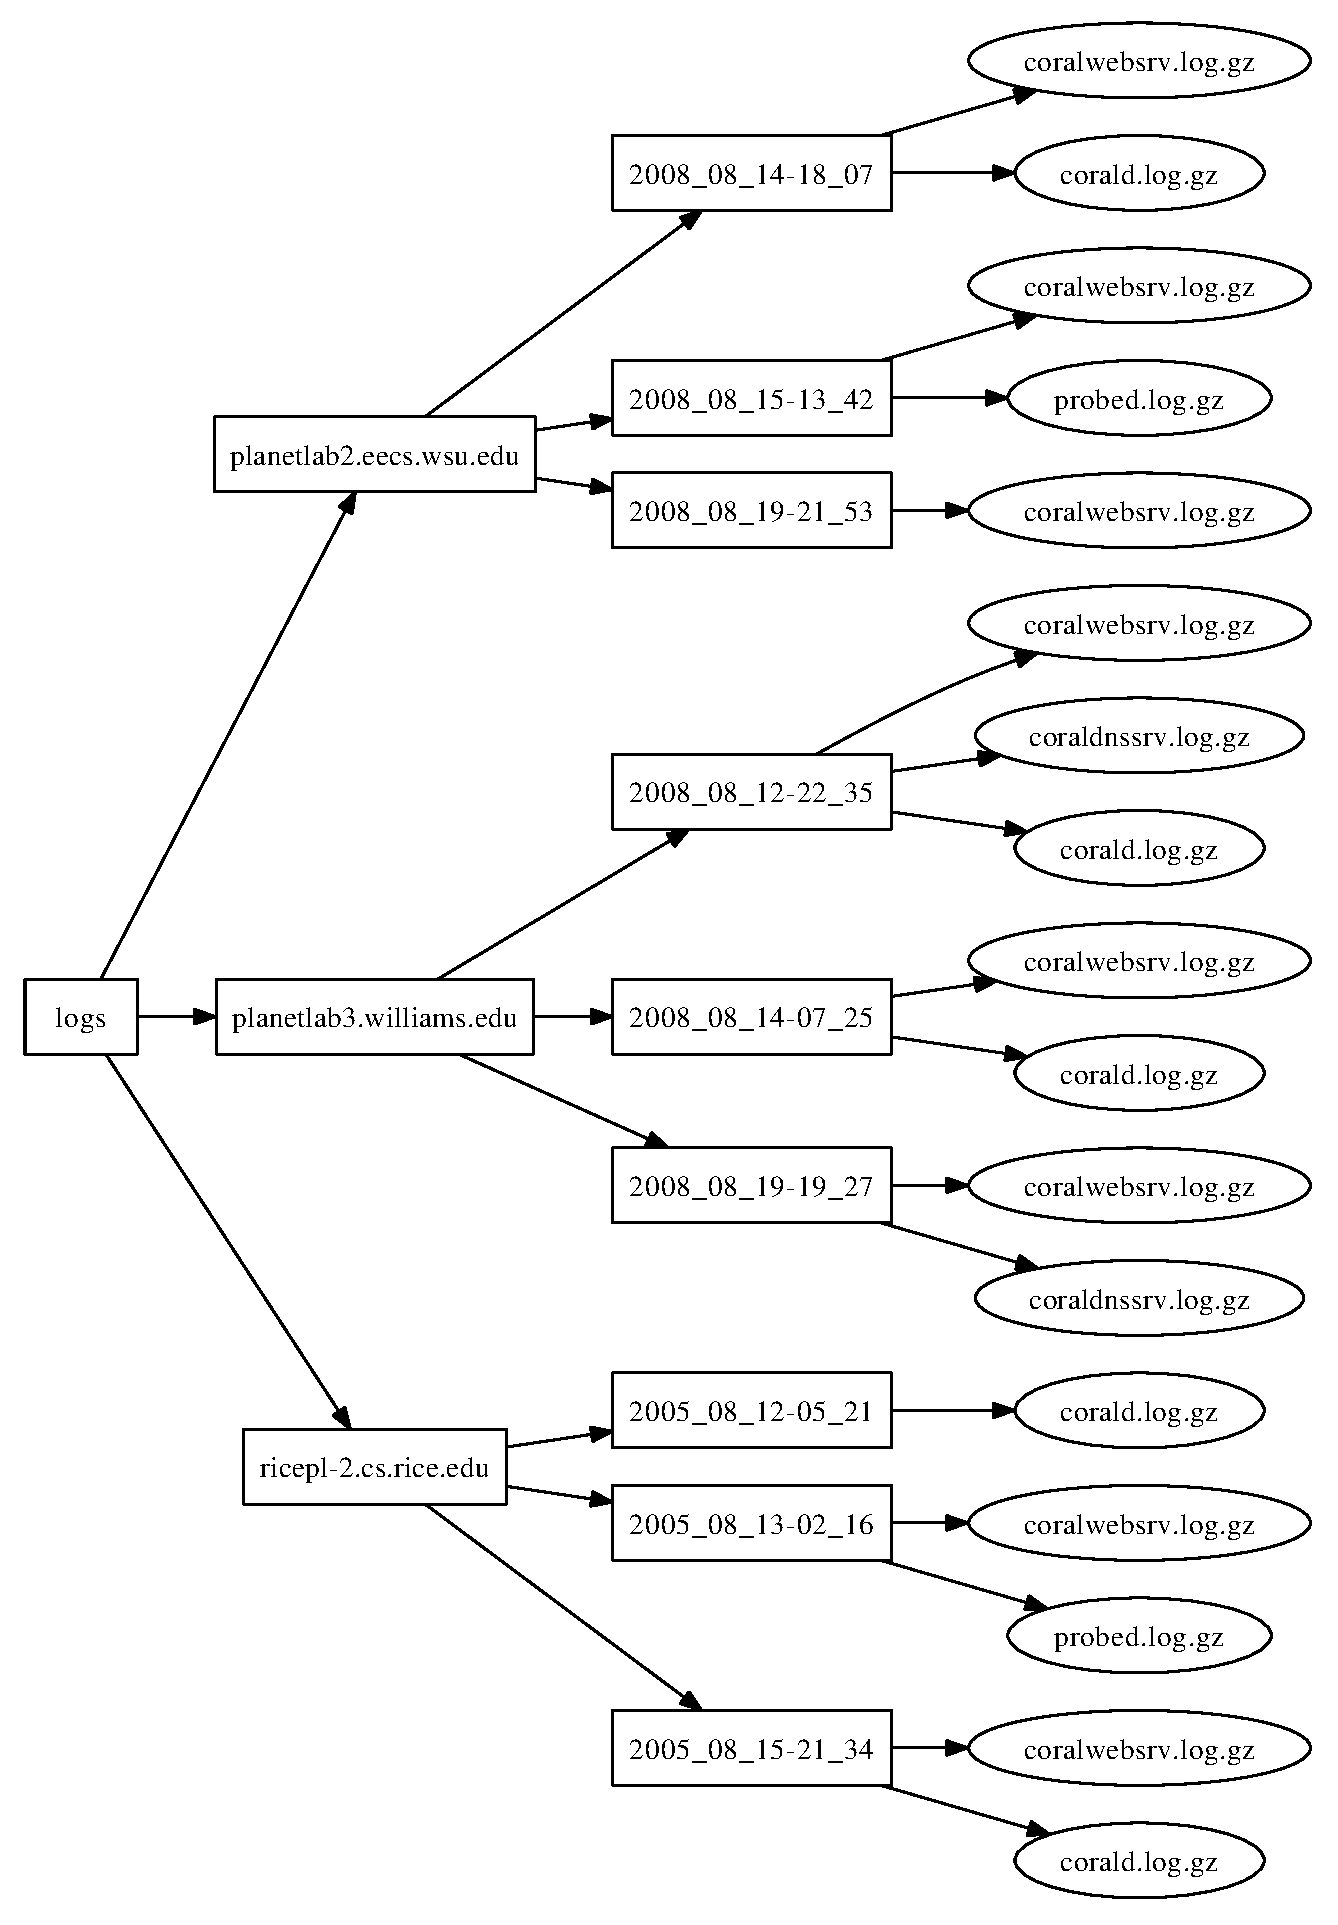
\epsfig{file=coral-structure.eps, width=0.9\columnwidth}
\caption{Coral system log data.}
\label{fig:coral-pic}
\end{figure}

\section{\forest{} Design}
\label{sec:review}

\forest{} is a domain-specific language embedded within Haskell using the
Template Haskell extension mechanism~\cite{metahaskell}.  In a typical
\forest{} description, \forest{} declarations will be interleaved with ordinary
Haskell declarations.  To introduce new \forest{} declarations in amongst
Haskell declarations,
the programmer simply opens the \forest{} sublanguage scope:
\begin{code}
[forest| 
  ... forest declarations ...
|]
\end{code}

Once within the forest sublanguage, the programmer will write declarations
that look and feel very much like extended Haskell type declarations.
Each such type declaration serves three purposes: (1) it specifies how the user
expects some fragment of the file system to appear, (2) it describes
the structure of the in-memory {\em representation} of that 
file system fragment when it is read into a Haskell program, and (3) it describes 
the structure of the {\em metadata} that is associated with reading the file system
fragment into the Haskell program.  As we explain the different features of \forest{}, 
readers should keep these three different aspects of \forest{} descriptions in mind.  
The effectiveness of our design comes in part due to the fact that these three 
elements may all be specified using a single compact description.  

Readers should also be aware
that the validity of every description is defined relative to a 
{\em current path} or {\em current position} within the file system.  As 
the system interprets a description against the file system, the current path
will change from one directory or file path to the next.  In general, descriptions
do not assume that the current path is a valid path in the file system.  When the current
path is invalid, a description will generally\footnote{The \cd{Maybe} constructor,
discussed later, is an example of an exception to the general rule.} 
register an attempt to load from that
path as an error in the associated metadata structure.

\subsection{Simple Files}
\label{sec:basics}

The basic building blocks of any file system are the files themselves.  To get started,
\forest{} provides several different ways to describe a file at the current position.  The simplest
way is to choose from a collection of standard, built-in file descriptions:\footnote{Recall that
any text following \cd{--} is a comment in Haskell.} 
\noindent
\begin{code}
[forest| 
  type MyText = File Ptext   -- a text file
  type MyBin = File Pbin     -- a binary file
  type Whatever = File Pany  -- any file at all
|]
\end{code}
Each such declaration creates an identifier ({\it e.g.,} \cd{MyText}) that can be used in other
more complex descriptions later.  It also generates several utility functions that may
be used in the surrounding Haskell code, including functions 
for loading files that match the given description.  

Descriptions such as \cd{MyText} are useful when the user neither knows or cares much about
the internal structure of the given file.  On the other hand, when the user does know and does
care about the internal structure of a file, he or she will want to describe that structure,
and will be able to do so using \padshaskell{}.  \padshaskell{} is another sublanguage,
based on the PADS family of parser 
generators~\cite{fisher+:pads,fisher+:popl06,mandelbaum+:pads-ml}, but 
designed for use with Haskell and \forest{}.  \padshaskell{} declarations are introduced
within the pads scope:
\noindent
\begin{code}
[pads| 
  ... pads declarations ...
|]
\end{code}
These declarations are capable of generating parsers that may be referred
to later within \forest{}.  For example, it is straightforward to use \padshaskell{} to generate
a parser for student files such as the one shown in Figure~\ref{fig:student-file-example}
(see the appendix for its definition).
Assuming that the parser for the file is named \cd{Student} and that it takes a single string parameter
(\cd{n}, the student name), we can use it within \forest{} as follows.
\begin{code}
[forest| 
  type SFile (n::String) = File (Student n) 
|]
\end{code}
Using \padshaskell{} parsers in \forest{} not only helps specify the intended grammatical structure
of a file, but it also generates a structured in-memory representation for Haskell programmers
to traverse, query or otherwise manipulate.  Indeed, \padshaskell{} and \forest{}
were designed to work seemlessly together.  From the perspective of the Haskell
programmer traversing an in-memory data structure, there is effectively
no difference between iterating over files in a directory or
structured sequences of lines or tokens within a file.

While the design of \padshaskell{} is interesting in its own right, the rest of this
paper focuses on \forest{}.  Henceforth, the reader should assume
any unadorned declarations 
occur within the \forest{} scope \cd{[forest| ... |]} unless otherwise noted.
The reader should also assume any declarations prefixed by \cd{>} are ordinary
Haskell declarations.

\subsection{File Modifiers}
\label{sec:file-modifiers}

Some files need processing by a utility before they can be used.  A typical
example is a compressed file such as the gzipped log files in the Coral
example shown in Figure~\ref{fig:coral-pic}.  \forest{} allows users to describe such 
files using various modifiers.  For example, if \cd{CoralInfo} is a \padshaskell{}
description of a Coral log file then the following describes a gzipped log file.
\begin{code}
type CoralLog = Gzip (File CoralInfo)
\end{code}
Likewise, suppose \cd{logs.tar.gz} is a gzipped tar file and suppose also that 
\cd{AllLogs} describes the directory of log files that \cd{logs.tar} expands
to.  In this case, the following description will describe the contents of
\cd{logs.tar.gz} properly.
\begin{code}
type CoralLogs = Gzip (Tar AllLogs)
\end{code}

\subsection{Symbolic Links}
\label{sec:symlinks}

When symbolic links are present in the file system described,
the default behavior is to read through the symbolic links to their
targets.  Hence, the behavior of \forest{} will be intuitive to programmers who
are used to working in a standard UNIX-like environment.  In addition, however, it is possible
for a programmer to explicitly specify that she expects a symbolic link in a particular
position.  To do so, the programmer will use the \cd{SymLink} base type.  For
example:
\begin{code}
type MyFile = SymLink
\end{code}
In \forest{}, any file system object may be described in multiple different ways.
Hence, in the case of symbolic links, it is possible to use one declaration to
specify the fact that an object is a symbolic link, and a second declaration to specify
the nature of the target that link ({\em e.g.,} the target is a text file).  We will see such 
a specification in later subsections.

\subsection{Simple Directories}
\label{sec:simple-directories}

The simplest way to specify the contents of a directory is to use
a record-like declaration.  For example, to specify the root directory
of the student repository in Figure~\ref{fig:student-pic}, we might use
the following declaration.  This declaration assumes that we have already
defined \cd{Class n}, a parameterized description that specifies
the structure of a directory holding data on the class of year \cd{n},
and \cd{Grads}, a description that specifies the structure of the directory holding
all graduated classes.   
\begin{code}
type All = Directory
  \{ seniors is "classof11" :: Class 11
  , juniors is "classof12" :: Class 12
  , grads is "graduates" :: Grads
  , notes is "README" :: File Ptext
  \}
\end{code}
Above, each field of the record has three components:  (1) a label
name ({\it e.g.,} seniors or juniors), (2) a file or directory name
({\it e.g.,} "classof11" or "classof12"), and (3) a \forest{} subdescription
for the contents of the named object ({\it e.g.,} \cd{Class 11} or \cd{Grads}
or \cd{File Ptext}).

With simple descriptions like this one, it is common for users to want
the label to be the same as the name of the file.  In such a case, users
may write the following abbreviated description:
\begin{code}
type All = Directory
  \{ classof11 :: Class 11
  , classof12 :: Class 12
  , graduates :: Grads
  , notes is "README" :: File Ptext
  \}
\end{code}
Above, the name of the label is used as the expected file name.  We did not
shorten \cd{notes is "README"} to \cd{README} because labels must start
with a lowercase letter in Haskell.

\paragraph*{Matching.}
In order for a file system object to match a description like the one above, it must be a
directory and each field of the record must match.  A field matches when the given
file name ({\em e.g.,} \cd{"README"}) is concatenated to the current path and the 
object at that new path matches the field's subdescription.

It is possible for the same file system object to to match multiple different fields of a description at
the same time.  For example, if "README" were a symbolic link that pointed to a text file, one 
might want to specify that using a pair of declarations:
\begin{code}
type All = Directory
  \{ ...
  , link is "README" :: SymLink
  , notes is "README" :: File Ptext
  \}
\end{code}

It is also possible for a directory to contain a number of objects that go unmatched by
a description.  We made the design choice to allow extra items in
a directory because we found it common for directories to contain files that users
simply do not care much about.  For example,
if programmers do not need to extract information out of the README file and
users do not really care whether it exists or not, one might well choose
to omit it from the description.  One might be concerned that this design choice makes it difficult to specify
the absence of files (as opposed to their presence), which can be important
for security purposes in some cases.  However, we will see shortly that in the
uncommon case that programmers want to specify absence information, they can
do so using constraints.

When a directory does match a record declaration like this one, 
\forest{} provides utilities to read the directory in
to memory and generate a convenient programmatic representation for it.  
In this case, the type of the in-memory representation is a record type
with labels \cd{seniors}, \cd{juniors}, {\em etc.} and with field types
generated from the associated \forest{} subdescriptions \cd{Class}, \cd{Grads},
{\em etc.}  When the same object is described in two different ways, one may
get two different in-memory representations of it.  For instance, in the example above,
the \cd{link} field will hold a representation of the filepath that describes the target of the
symbol link whereas the \cd{notes} field will hold a representation of the \cd{README}
file itself ({\em i.e.,} a string of characters).

When a directory does not match a record declaration, \forest{} will
construct representations for the subparts that do match and will insert dummy values
into the parts that do not match.  \forest{} will also record all errors encountered in the
matching process in the object metadata.

\subsection{Computed and Approximate Paths}
\label{sec:computed-pathes}

Both of the above descriptions are a good start for our application, but neither
are ideal.  Every year, the directory for the graduating seniors 
({\em i.e.,} \cd{classof11}) gets moved into the graduates directory,
the juniors get promoted to seniors and a new junior class gets created.
As it stands, this means we would also have to edit our description every year.
An alternative is to parameterize our description with the current year and
to construct the appropriate file names.  If we follow this strategy,
we might arrive at the following specification for the top-level student directory:
\begin{code}
> mkclass y = "classof" ++ (toString y)
\mbox{}
type All (y::Integer) = Directory
  \{ seniors is <|mkclass y|> :: Class y
  , juniors is <|mkclass (y+1)|> :: Class <|y+1|>
  , graduates :: Grads
  , notes is "README" :: File Ptext
  \}
\end{code}
%\begin{code}
%type All (sy::String, jy::String) = Directory
%  \{ seniors is <|"classof" ++ sy|> :: Class
%  , juniors is <|"classof" ++ jy|> :: Class
%  , graduates :: Grads
%  , notes is "README" :: File Ptext
%  \}
%\end{code}
In general, \cd{<|...|>} can be used to escape back in to
Haskell to perform arbitrary computations.  Note also that any description
may be parameterized by specifying a legal Haskell identifier and its type.
Parameterized specifications may be used by supplying their arguments
in the usual way.  When arguments are simple constants or variables,
they may be supplied directly.  When arguments are more complex
computed expressions, it is necessary to use explicit escapes back 
in to Haskell.

As repositories evolve over time, naming conventions may change.
Alternatively, programmers simply may not care to specify certain names
exactly.  To accomodate these possibilities, \forest{} includes mechanisms
for approximate naming of files.  For example, in each class, there may
(or may not) be some number of students that have withdrawn from the
program, transferred to a different Princeton program on gone on
temporary leave.  Over the years, slightly different directory names
have been used to represent these situations.  Given this circumstance,
we can use the following declarations to describe the class directory.
\reminder{dpw: I edited out some of the withdrawn RE options to make it
fit on a line.}\reminder{jnf:how about making all of them two characters long (``tr'', ``wd'', ``lv'')?}
\begin{code}
> transRE = RE "TRANSFER|Transfer"
> leaveRE = RE "LEAVE|Leave"
> wdRE    = RE "WITHDRAWN|WITHDRAWAL|Withdrawn"
\mbox{}
type Class (y::Integer) = Directory
  \{ bse is <|"BSE" ++ (toString y)|> :: Major
  , ab  is <|"AB"  ++ (toString y)|> :: Major   
  , trans matches transRE :: Maybe Major      
  , wd matches wdRE :: Maybe Major
  , leave matches leaveRE :: Maybe Major 
  \}
\end{code}
A field with the form \cd{<label> matches <regexp> :: T}
finds the set of paths in the files system that match \cd{currentPath/} \cd{<regexp>}.
If there are zero or one matches, the \cd{matches} form acts like the \cd{is} 
form.\footnote{Recall that when 
there are zero matches, the \cd{is} form attempts to match the type \cd{T} 
against a non-existant file system object at a non-existant path.  This may or may not be
an error, depending on \cd{T}.  The matches form constructs a non-existant path
and behaves the same way.}  If there is more than one match, one of the many matches
is selected non-deterministically, a multiple match error is registered in the metadata,
and matching once again continues as in the \cd{is} form.

In this example, the \cd{matches} form is combined with the \cd{Maybe T} constructor.
\cd{Maybe T} succeeds and returns \cd{None} when the current path is not a path in the
file system.  \cd{Maybe T} also succeeds, returning \cd{Just v} for some \cd{v},
when applied to an object that matches \cd{T} at the current path.  \cd{Maybe T} 
registers an error in the metadata when the current path exists but 
the object at the current path does not properly match \cd{T}.

\subsection{Comprehensions}
\label{sec:comprehensions}

Record directories allow programmers to specify a fixed number of file system objects.
Comprehensions, on the other hand, allow programmers to specify arbitrary numbers
of file system objects.  As an example, we might specify the contents of the
\cd{Grads} directory from Figure~\ref{fig:student-file-example} as follows.
\reminder{dpw: changed Prelude.take into take below for space reasons.}
\reminder{dpw: perhaps the definition of getYear should use Haskell composition "." instead
of all the parens? Also, I changed the type of the Class parameter to an integer. Hence, I needed the toInteger conversion -- it wasn't obvious to me from the Haskell docs if in fact toInteger will
convert from a string to an integer. In the current Students2.hs (Oct. 23), all comprehensions
are nested within records.  I unnested here. I can imagine syntax is a possible issue with doing
that but not semantics.  The record wrapper does seem unnecessary overhead for the programmer.
(But really, it just helps me with the explanation here, because it makes comprehensions orthogonal.}
\begin{code}
> cYear s = 
>   toInteger (reverse (take 2 (reverse s)))
> cRE = RE "classof[0-9][0-9]"
\mbox{}
type Grads = 
  [c :: Class <|cYear c|> | c <- matches cRE]
\end{code}
In the specification above, \cd{Grads} is a directory that contains a number of
\cd{Class} subdirectories with names \cd{c} that match the regular expression
\cd{cRE}.  The Haskell function \cd{cYear} extracts the last two digits from the
name of the directory, converts the string digits to an integer year, and passes
the year to the underlying \cd{Class} specification.
More generally, comprehensions have the following form.
\begin{code}
[path :: T | id <- gen, pred]
\end{code}
Here, \cd{id} is bound to each of the strings generated by the \cd{gen},
which may be a \cd{matches} function (used to match against the files
at the current path) or may be some other list computed in Haskell. The allowed
\cd{id}s may be filtered by \cd{pred} and they may be used in the computation
\cd{path}.  Each such computed path is concatentated to the current path and
used to match a file system object with type \cd{T}.  The predicate and path
computation may also use the path metadata by referring to the variable
\cd{id_md}, which will be in scope.  The in-memory representation of a comprehension
is a list.

Another example of a comprehension occurs in specification the \cd{Major} 
directory.  These directories contain a list of student files, and one additional
template file named \cd{sss.txt} or \cd{sxx.txt}.  The declaration below
specifies all the student files except the template files.  Note that it uses
a glob pattern as opposed to a regular expression
to describe a set of text files.\footnote{A glob pattern
is a pattern used to describe file paths in UNIX-based systems.  Such patterns include
constant strings and wildcards \cd{*} and \cd{?}.} 
\begin{code}
> tpl s = (s == "sss.txt") || (s == "sxx.txt")
> txt = GL "*.txt"
\mbox{}
type Major =   
  [ s :: File (Student <|getName s|>) 
  | s <- matches txt, <|not (tpl s)|>]
\end{code}

\subsection{Attributes and Constraints}
\label{sec:constraints}

Every file system object has a number of attributes associated with it.  In general,
if a \forest{} identifier \cd{id} refers to a path, the attributes for the object at that
path are available through the identifier named \cd{id_att}. Figure~\ref{fig:metadata-components}
lists a set of functions that extract useful information from metadata structures.
Below, metadata functions used to write a universal description.
Notice that the description also happens to be recursive, another useful feature of
\forest{}.  In the case that a symbolic link creates a cycle in the file system, the Haskell
in-memory representation will be a (lazy) infinite data structure. 
\reminder{jnf: the preceding remark is only true if the symbolic link points to a directory, right?}
\begin{code}
type Universal = Directory 
  \{ asc is [ f :: File Ptext   
           | f <- matches (GL "*"), 
            <|get_kind f_att == AsciiK|>]
  , bin is [ b :: File Pbinary
           | b <- matches (GL "*") 
           where <|get_kind b_att == BinaryK|>]
  , dir is [ d :: Universal  
           | d <- matches (GL "*") 
           where <|get_kind d_att == DirectoryK|>]
  , sym is [s :: SymLink      
           | s <- matches (GL "*") 
           where <|get_sym s_att == True|>]
  \}
\end{code}

Attributes are also commonly used in {\em constraints}.  For example, if a user
wants to ensure that all her text files are private,
she might replace the use of \cd{File Ptext} in a description with the following
\cd{PrivateFile} definition.  
\reminder{dpw: The following two examples need to be tested to ensure correctness.}
\begin{code}
type PrivateFile = 
  File Ptext 
    where <|get_modes this_att == "-rw-------"|>
\end{code}
Here, the keyword \cd{where} introduces a constraint
on the underlying type.  If a constraint evaluates to false, an error
is registered in the metadata.  Within the constraint, \cd{this} refers to the representation 
of the underlying object, \cd{this_att} refers to its attributes and \cd{this_md} refers
to its metadata.

Another use for constraints involves specifying emptiness conditions or conditions that
certain files do not appear in certain places.  As an example, one might want to specify
that no binaries appear in a directory given to an untrusted user as scratch space.
The description below registers an error whenever a binary file appears in the described
directory. 
\begin{code}
type NoBin =
  [ b :: File Pbinary 
  | b <- matches (GL "*"), 
  <|get_kind b_att == BinaryK|> ]
  where <|List.length this == 0|>
\end{code}

\begin{figure}
\begin{center}
\begin{tabular}{l|l}
function name &  information \\
\hline
\cd{get_group} & object group\\
\cd{get_kind} & the sort of file or directory \\
\cd{get_modes} & permission string\\
\cd{get_owner} & object owner\\
\cd{get_size} & object size \\
\end{tabular}
\end{center}
\caption{Selected file attribute functions}
\label{fig:metadata-components}
\end{figure}

\subsection{Representation Coercions}
\label{sec:transforms}

One of the benefits of using \forest{} is that every description serves multiple purposes:
(1) it specifies the structure of the file system on disk, (2) it specifies structure of in-memory
representations of the file system, (3) it generates type declarations describing those in-memory
structures, and (4) it generates data structures representing error conditions and other meta data.
\reminder{jnf: above, we identified three things generated from descriptions...}

Sometimes, however, it is useful to be able to override the default structure of the generated items.
In particular, we have found that programmers occasionally want the representation of their in-memory data
structured differently than the default.  In order to give programmers choice on this matter when they want it,
\forest{} permits them to use {\em representation coercions} within a description.  As an example, consider
again the definition of \cd{Major} from subsection~\ref{sec:comprehensions}.  In that definition, the
in-memory representation of the set of majors is a list of \cd{(name.txt,filecontents)} pairs.  A more convenient
representation for programming, however, is likely a map from \cd{names} to \cd{filecontents}.  Assuming
\cd{MapName} is the coercion from lists to maps suggested, 
we insert it into the description as follows.\reminder{dpw: can we put the definition of mapname in?  I don't know
how to write it.  I can't find Kathleen's email with some mention that any Builder something something toList
function something something is how you write these functions.}
\begin{code}
type Major = 
  MapName [ s :: File (Student <|getName s|>) 
          | s <- matches txt, <|not (tpl s)|>]
\end{code}
While programmers may build their own custom coercions as above, \forest{} does supply a set of 
generic, built-in coercions as well such as \cd{Map} (convert to a map from file name to contents)
and \cd{Set} (convert to a set of contents).

\subsection{Putting it all together}

The previous subsections explain most of the interesting features of \forest{}.
These features are put to work in Figures~\ref{fig:student-description}
and~\ref{fig:coral-description}.  A set of other descriptions are available on 
the \forest{} web site~\cite{forest-web-site}.

\begin{figure}
\begin{code}
[forest|
 \kw{data} PrincetonCS (y::Integer) = \kw{Directory}
   \{ notes   \kw{is} "README" :: Text
   , seniors \kw{is} <|mkClass y    |> :: Class y
   , juniors \kw{is} <|mkclass (y+1)|> :: Class <|y+1|>
   , graduates :: Grads
   \}
\mbox{}
 \kw{data} Class (y::Integer) = \kw{Directory}
   \{ bse \kw{is} <|"BSE" ++ (toString y)|> :: Major
   , ab  \kw{is} <|"AB"  ++ (toString y)|> :: Major   
   , trans \kw{matches} transRE :: Maybe Major      
   , withd \kw{matches} wdRE    :: Maybe Major
   , leave \kw{matches} leaveRE :: Maybe Major 
   \}
\mbox{}
 \kw{type} Grads = 
   [c :: Class <|getYear c|> | c <- \kw{matches} cRE]
\mbox{}
 \kw{type} Major = Map
    [ s :: File (Student <|dropExtension s|>) 
    | s <- \kw{matches} txt, <|not (template s)|>]
|]
\end{code}
% \mbox{}
% [pads|
%   \kw{data} Student (name::String) = ...
% |]
% \mbox{}
% toStrN i n = (replicate(n - length(show i)) '0') 
%              ++ (show i)
% mkClass y = "classof" ++ (toStrN y 2)
% getYear s = 
%   toInteger (reverse (take 2 (reverse s)))
% template s = s `elem` ["sss.txt", "sxx.txt"]

% transRE = RE "TRANSFER|Transfer"
% leaveRE = RE "LEAVE|Leave"
% wdRE    = RE "WITHDRAWN|WITHDRAWAL|Withdrawn"
% cRE     = RE "classof[0-9][0-9]"
% txt     = GL "*.txt"
\caption{\forest{} student description -- out of date (nov 1)}
\label{fig:student-description}
\end{figure}

\begin{figure}
\begin{code}
[forest|
  \kw{data} Log = \kw{Directory}
    \{ log \kw{is} coralwebsrv :: Gzip (File CoralLog) \}
  \kw{type} Site  = [ d :: Log  | d <- \kw{matches} time ]
  \kw{type} Coral = [ s :: Site | s <- \kw{matches} site ]
|]
\end{code}
\vskip -5pt
%\mbox{}
%[pads|
%  \kw{type} CoralLog = ...
%|]
%\mbox{}
%coralwebsrv = "coralwebsrv.log.gz"
%time = RE "[0-9]\{4\}(_[0-9]\{2\})\{2\}-[0-9]\{2\}_[0-2]\{2\}"
%site = RE "[^.].*"

\caption{\forest{} coral description -- out of date (nov 1)}
\label{fig:coral-description}
\end{figure}

\section{Programming with \forest{}}
\label{sec:exp}

\begin{figure}
\begin{code}
log_load :: FilePath -> IO (Log, Log_md),
site_load :: FilePath -> IO (Site, Site_md)
top_load :: FilePath -> IO (Top, Top_md),
\end{code}
\caption{Load functions for Coral}
\label{fig:coral-load}
\end{figure}

\begin{figure}
\begin{code}
data Log = Log { log :: CoralLog }
newtype Site = Site [(String, Log)]
newtype Top = Top [(String, Site)]
\end{code}
\caption{Representation types for Coral}
\label{fig:coral-rep}
\end{figure}

\begin{figure}
\begin{code}
data Log_inner_md = 
  Log_inner_md { log_md :: (Forest_md, CoralLog_md) }
type Log_md = (Forest_md, Log_inner_md)
type Site_md = (Forest_md, [(String, Log_md)])
type Top_md = (Forest_md, [(String, Site_md)])
\end{code}
\caption{Metadata types for Coral}
\label{fig:coral-md}
\end{figure}


\reminder{jnf: TODOs
\begin{itemize}
\item Format of coralwebsrv.log.gz is not currently explained anywhere.
\item Must explain the structure of entries for the top-k example.
\end{itemize}}

Most \forest{} programs work in two phases. In the first phase they
use \forest{} to load certain portions of the file system into memory,
and in the second phase they use an ordinary Haskell function to
traverse the in-memory representation of the data (or its associated
metadata) and compute the desired result.

To facilitate this style of programming, the \forest{} compiler
generates a several Haskell functions and types from every \forest{}
description.  It generates a \emph{load function}, which traverses the
file system and reads the files, directories, and symbolic links
mentioned in the description into a structured object in memory; it
generates a Haskell type for the in-memory \emph{representation} of
the data produced by the load function; and it generates a Haskell
type for the \emph{metadata} associated with the representation. For
example, from the descriptions for CoralCDN logs in
Figure~\ref{fig:coral-description}, the compiler generates the load
functions in Figure~\ref{fig:coral-load}, the representation types in
Figure~\ref{fig:coral-rep}, and the metadata types in
Figure~\ref{fig:coral-md}. Note that the structure each of these
artifacts closely corresponds to the structure of the \forest{}
description that generated them. This makes it easy for programmers to
write programs against these \forest{}-generated artifacts.

As a simple example, consider the \cd{Top} description from
Figure~\ref{fig:coral-description}. The \cd{top\_load} function takes
a path as an argument and produces the representation and metadata
obtained by loading each of the site directories contained in the
directory at that path:
%
\begin{code}
(rep,md) = 
  unsafePerformIO $ (top_load "/var/log/coral")
\end{code}
% $
Because \cd{Top} is a comprehension, both \cd{rep} and \cd{md} are
structured as lists. More specifically, \cd{rep} has the form,
\begin{code}
Top [("planetab2.eecs.wsu.edu", Site [...]),
     ("planetlab3.williams.edu", Site [...]), ...]
\end{code}
where the list contains pairs of names of subdirectories and
representations for the data loaded from those directories. The
metadata is a pair consisting of a generic header of type
\cd{Forest\_md} and a list of pairs of names of subdirectories and
their associated metadata. The header records aggregate information
about any errors encountered during loading as well as the file system
attributes of each file, directory, or symbolic link loaded from the
file system:
%
\begin{code}
Forest_md 
  \{ numErrors = 0, 
    errorMsg = Nothing, 
    fileInfo = FileInfo
      \{ fullpath = /var/log/coral, 
        owner = alice, group = staff, size = 102, 
        access_time = Fri Nov 19 01:47:09 2010, 
        mod_time = Thu Nov 18 20:42:37 2010, 
        read_time = Fri Nov 19 01:47:28 2010, 
        mode = drwxr-xr-x, isSymLink = False, 
        kind = Directory \} \},
[("planetlab2.eecs.wsu.edu", Forest_md \{...\}),
 ("planetlab3.williams.edu", Forest_md \{...\}), ...]
\end{code}
%

Using these functions and types, it is easy to formulate many useful
queries as simple Haskell programs. For instance, to count the number
of sites we can simply compute the length of the nested list in
\cd{rep}:
%
\begin{code}
num_sites = case rep of Top l -> List.length l 
\end{code}
%
More interestingly, to calculate the time when statistics were last
reported for each site, we can zip the lists in \cd{rep} and \cd{md}
together and project out the site name and the \cd{mod_time} field
from each element in the resulting list of pairs:
%
\begin{code}
get_site = fst
get_mod (_,(f,_)) = mod_time . fileInfo $ f  
sites_mod () = 
  case rep,md of (Top rs, (_,ms)) -> 
    map (get_site *** get_mod) (zip rs ms)
\end{code}
% $
\reminder{jnf: do we want to show output? we'll have to be careful to
  sanitize the data.}

These simple examples show how \forest{} diminishes the distinction
between data represented on disk and in memory. After writing a
suitable \forest{} description, programmers can write programs that
work on file system data as if it were in memory. Moreover, because
Forest uses lazy I/O operations, many simple programs do not require
constructing an explicit representation of the entire directory being
loaded in memory---a good thing as the directory of CoralCDN logs
contains approximately 1GB of data!  Instead, the load functions only
read the portions of the file system that are needed to compute the
result---in this case, only the site directories and not the gzipped
log files contained within them.

As a final example, consider a program that computes the top-$k$
requested URLs from all CoralCDN nodes by size. The CoralCDN
administrators compute this statistic periodically to help monitor and
tune the performance of the system~\reminder{cite Mike's NSDI '10
  paper}. Here is its definition in Haskell (it uses several helper
functions such as \cd{get_sites} to project out various components of
\cd{rep}):
%
\begin{code}
topk k = 
  take k $ sortBy descBytes $ toList $
  fromListWith (+)
    [ (get\_url e, get\_total e)
    | (site,sdir) <- get\_sites rep,
      (datetime,ldir) <- get\_dates sdir,
      e <- get\_entries ldir,
      is\_in e ]
\end{code}
% $
Reading this program inside-out, we see that it first uses a list
comprehension to iterate through \cd{rep}, collecting up the
individual log entries in the \cd{coralwebsrv.log.gz} file for
incoming requests and projecting out the URL requested and the total
size of the request. It then adds up the sizes of all requests for the
same URL using the \cd{fromListWith} function from the \cd{Data.Map}
module. Next, it sorts the entries in descending order. Finally, it
returns the first $k$ entries of the list as the final result.
%
\reminder{jnf: compare with the hand-written Python program Mike
  actually uses? Highlight difficulties of dealing with large number
  of huge files?}

\section{Tools}
\label{sec:tools}
\begin{itemize}
\item tar, ...
\item Graph representation giving status
\item ??
\end{itemize}


\section{Implementation}

\begin{itemize}
\item explain implementation components: quasi-quoting, template haskell, etc.
\item explain generic programming strategy
\item evaluated performance: lazy vs. not? -- we need a graph
\end{itemize}

\section{A Core Calculus for \forest{}}
\label{sec:exp}
\renewcommand{\bnfdef}{\ensuremath{\mathord{::=}}}
\newcommand{\slsh}{\ensuremath{\mathord{\textsf{/}}}}
\newcommand{\File}[1]{\ensuremath{\mathsf{File}(#1)}}
\newcommand{\Dir}[1]{\ensuremath{\mathsf{Dir}(#1)}}
\newcommand{\Link}[1]{\ensuremath{\mathsf{Link}(#1)}}
\newcommand{\Set}[1]{\ensuremath{\{ #1 \}}}
\newcommand{\Map}[1]{\ensuremath{\{\!\mid #1 \mid\!\}}}
\newcommand{\PNil}{\ensuremath{\bullet}}
\newcommand{\PCons}[2]{\ensuremath{#1\,\textsf{/}\,#2}}
\newcommand{\Just}[1]{\ensuremath{\mathsf{Just(#1)}}}
\newcommand{\Nothing}{\ensuremath{\mathsf{Nothing}}}
\newcommand{\True}{\ensuremath{\mathsf{True}}}
\newcommand{\False}{\ensuremath{\mathsf{False}}}
\newcommand{\fn}[2]{\ensuremath{#1(#2)}}
\newcommand{\Sk}{k^{\tau_m}_{\tau_r}}
\newcommand{\SAdhoc}[1]{\ensuremath{\mathsf{Adhoc}({#1}^{\tau_m}_{\tau_r})}}
\newcommand{\SPred}[1]{\ensuremath{\mathsf{Pred}(#1)}}
\newcommand{\SPath}[2]{\ensuremath{#1 \mathrel{::} #2}}
\newcommand{\SPair}[3]{\ensuremath{\langle #1 {:} #2, #3 \rangle}}
\newcommand{\SOption}[1]{\ensuremath{#1?}}
\newcommand{\SSetComp}[3]{\ensuremath{\{ #1 \mid #2 \in #3 \}}}
\newcommand{\Env}{\ensuremath{\mathcal{E}}}
\newcommand{\ENil}{\ensuremath{\bullet}}
\newcommand{\yields}{\ensuremath{\rightsquigarrow}}
\newcommand{\valid}[1]{\ensuremath{\mathit{valid}(#1)}}
\newcommand{\typ}[1]{\ensuremath{\mathit{#1}}}
\newcommand{\meta}{\typ{meta}}
\newcommand{\REP}{\ensuremath{\mathit{REP}}}
\newcommand{\PD}{\ensuremath{\mathit{PD}}}
\newcommand{\pd}[1]{\ensuremath{(#1)~\mathit{pd}}}
\newcommand{\eval}[1]{\ensuremath{\mathsf{eval}(#1)}}
\newcommand{\ptext}{\ensuremath{\mathsf{Txt}}}
\newcommand{\pbin}{\ensuremath{\mathsf{Bin}}}
\newcommand{\pany}{\ensuremath{\mathsf{Any}}}
\newcommand{\att}{\ensuremath{\mathsf{a}}}
\newcommand{\defaultatt}{\ensuremath{\att_{\mathsf{df}}}}
\newcommand{\repty}[1]{{\cal R}[\![ #1 ]\!]}
\newcommand{\mdty}[1]{{\cal M}[\![ #1 ]\!]}
\newcommand{\checkk}[3]{\fn{\mathit{check}}{#1,#2,#3}}

In order to capture the essence of \forest{}'s semantics, we have
defined an idealized core calculus.  This calculus has helped us
design various aspects of the \forest{} language itself and provides
compact means by which we may communicate the central, orthogonal
concepts to others.  It is inspired by classical ({\em i.e.,} not
separating, substructural or ambient) unordered tree logics, though
customized for our particular needs.

\paragraph*{File system model and specification syntax.}
Figure~\ref{fig:calculus-syntax} presents the formal file system model.  
In our model, file paths $r$ are
sequences of string names\footnote{For simplicity, we ignore the special path
elements ``..'' and ``.''.  Adding these elements
requires path normalization in the semantics, which, while easily
achievable, does not shed light on interesting design elements.} 
and file systems $F$
are finite partial maps from paths to pairs of file attributes $\att$
and file system contents $T$.  We leave the attribute records $\att$ 
unspecified, but they should include the usual elements: owner, group,
date modified, {\it etc.}  We write $\defaultatt$ for the dummy or
default attribute record where necessary.
A $T$ may be a file $\File{n}$ (with underlying string contents $n$),
a directory $\Dir{ \Set{n_1,\dots,n_k} }$ (with contents named 
$n_1, \ldots, n_k$) or a symbolic link $\Link{r}$ (where $r$ is the
path linked to).  

A file system model $F$ is only {\em well-formed} when it is tree-shaped,
with directories forming internal nodes and files and symbolic
links the leaves.  More formally, the following conditions must hold:
\begin{itemize}
\item The domain of $F$ must be prefix-closed.
\item If $F(r) = (\att,\Dir{ \Set{n_1,\dots,n_k} })$ then for $i=1,\ldots,k$,
$\PCons{r}{n_i} \in \dom{F}$.
\item  If $F(r) = (\att,\File{n})$ or $(m,\Link{r'})$ then 
there does not exist $n$ such that $\PCons{r}{n} \in \dom{F}$.
\end{itemize}

Figure~\ref{fig:calculus-syntax} also presents the syntax of
a simple computation language $e$ and our
file system specifications $s$.  The computation language $e$
contains values $v$, variables $x$, and some number of other
operations, which we leave unspecified.  An environment
$\Env$ maps variables to values.  A semantic function
$\eval{\Env,F,r,e}$ evaluates an expression $e$ in an
environment $\Env$, file system $F$, and at current path $r$,
producing a value $v$.

The simplest file system specifications are the constants
$k$, which range over basic specifications such as those for
text files (\ptext), binary files (\pbin), or any
file system object at all (\pany). 

\padshaskell{} specifications are modelled as
\SAdhoc{b} where $b$, a parser,  is a total
function from pairs of environments and strings to
values.  

For syntactic reasons, \forest{} itself combines specifications
for records and paths and also comprehensions and paths.
However, the calculus reveals that (dependent) records, paths 
and comprehensions
may all be understood as independent, orthogonal constructs.
The record specifications are modelled as a dependent pair,
written \SPair{x}{s_1}{s_2}, where $x$ may appear in $s_2$.
A path specification is written $\SPath{e}{s}$, where $e$ is
a path name (to be appended to the current path) and 
$s$ specifies the file system fragment at that path.  As an example,
a combined \forest{} record-and-path specification such as
\cd{\{c is "c.txt" :: C, dat is "d.txt" :: D c\}}
is written in the calculus as
$\SPair{x}{(\SPath{\mathtt{"c.txt"}}{C})}{(\SPath{\mathtt{"d.txt"}}{D\; x})}$.
A specification with the form $\SSetComp{s}{x}{e}$ is a comprehension where
$e$ is a set of values, $x$ is bound to each such value in turn, and
$s$, which may contain $x$, specifies a file system fragment for each
such $x$.  Again, a combined \forest{} comprehension-and-path
\cd{[x :: s | x <- e]} is modelled as the composition of two
orthogonal constructors ($\SSetComp{s_1}{x}{e}$ and $s_1 = \SPath{x}{s}$).

A predicate specifications $\SPred{e}$ succeeds
when $e$ evaluates to \True{} and fails when $e$ evaluates
to \False.  A \forest{} constraint of the form \cd{s where e}
is modelled in the calculus as a dependent pair with a predicate:
$\SPair{x}{s}{\SPred{e[x/\mathtt{this}]}}$

Finally, a maybe specification is written $\SOption{s}$ in the calculus.
 
\begin{figure}
\[
\begin{array}{rr@{\;}r@{\;}l}
\textit{Strings}        & n & \in & \Sigma^{\ast} \\[1ex]
\textit{Paths}          & r,s & \bnfdef & \PNil \mid \PCons{r}{n} \\[1ex]
\textit{Attributes}     & \att  & \bnfdef & \dots\\[1ex]
\textit{Filesystem}     & T  & \bnfdef & \File{n} \\
\textit{Contents}       &    & \bnfalt & \Dir{ \Set{n_1,\dots,n_k} }\\
                        &    & \bnfalt & \Link{r}\\[1ex]
\textit{Filesystems}    & F & \bnfdef & \Map{ r_1 \mapsto (\att_1,T_1), \dots r_k \mapsto (\att_k,T_k) }\\[1ex]
\textit{Values}         & v & \bnfdef & \att \bnfalt n \bnfalt r \bnfalt \True \bnfalt \False \bnfalt () \bnfalt (v_1,v_2) \\
                        &   & \bnfalt & \Just{v} \bnfalt \Nothing \bnfalt \{ v_1,\dots,v_k \}\\
\textit{Expressions}    & e & \bnfdef & x \bnfalt v \bnfalt \dots \\[1ex]
\textit{Environments}   & \Env & \bnfdef & \ENil \bnfalt E,x\mapsto v \\[1ex]
\textit{Specifications} & s & \bnfdef & \Sk \\
                        &   & \bnfalt & \SAdhoc{b}\\
                        &   & \bnfalt & \SPath{e}{s}\\
                        &   & \bnfalt & \SPair{x}{s_1}{s_2}\\
                        &   & \bnfalt & \SSetComp{s}{x}{e}\\
                        &   & \bnfalt & \SPred{e}\\
                        &   & \bnfalt & \SOption{s}\\[1ex]
\end{array}
\]
\caption{File systems and their specifications}
\label{fig:calculus-syntax}
\end{figure}

\paragraph*{Calculus Semantics.}
The calculus has a semantics in three parts, which represent the three different
artifacts generated by the \forest{} compiler from each specification.  The
first semantic judgement has the form $\Env;F;r \models s \yields v,d$.
Intuitively, this judgement states that in environment $\Env$ and file system
$F$, specification $s$ matches the file system fragment at current path $r$
and produces file system representation $v$ and metadata $d$.  This judgement
may also be viewed as a total function from $\Env$, $F$, $r$ and $s$ to the
pair $v$ and $d$.  The judgement is total because when file system fragments
fail to match the given specification, defaults are generated for the representation
$v$ and errors are recorded in the metadata $d$.  This design is preferable to
failing outright as it allows a programmer
to explore a file system fragment even when it contains errors, as is common
in ad hoc data repositories.  The second and third
semantic judgements characterize the shape of the representation and metadata
given a specification by giving their types.  They have the form $\repty{s} = \tau$ and
$\mdty{s} = \tau$, respectively.  The three sets of definitions obey the following
basic coherence property, where $\turn v : \tau$ states that value $v$ has type $\tau$.

\begin{proposition}
If $\Env;F;r \models s \yields v,d$ and
$\repty{s} = \tau_r$ and $\mdty{s} = \tau_m$
then $\turn v : \tau_r$ and $\turn d : \tau_r$ 
\end{proposition}


The semantics of our calculus is spelled out in Figure~\ref{fig:calculus-semantics} 
and \ref{fig:calculus-types}.

\begin{figure}
\[
\infrule
{ }
{ \Env;F;r \models \Sk \yields \checkk{\Sk}{F}{r} }
{}
\]

\[
\infrule
{ F(r) = (\att,\File{n}) \qquad 
  b(E,n) = v,d }
{ \Env;F;r \models \SAdhoc{b} \yields v,(\valid{d},(d,\att)) }
{ }
\]

\[
\infrule
{ %\begin{array}{l}
  F(r) = (\att,\Dir{\_}) \text{ or } F(r) = (\att,\Link{\_}) \qquad
  b(E,\epsilon) = (v,d)
  %\end{array} 
}
{ \Env;F;r \models \SAdhoc{b} \yields v,(\False,(d,\att)) }
{}
\]

\[
\infrule
{ 
  r \not\in \dom{F}  \qquad
  b(E,\epsilon) = (v,d)
}
{ \Env;F;r \models \SAdhoc{b} \yields v,(\False,(d,\defaultatt)) }
{}
\]

\[
\infrule
{ \Env;F;\eval{E,F,r,\PCons{r}{e}} \models s \yields v,d }
{ \Env;F;r \models \SPath{e}{s} \yields v,d }
{ }
\]

\[
\infrule
{ \begin{array}{c}
  \Env;F;r \models s_1 \yields v_1,d_1 \\
  \Env[x \mapsto v_1, x_d \mapsto d_1];F;r \models s_2 \yields v_2,d_2 \\
  v = (v_1,v_2) \qquad d = (d_1,d_2) 
  \end{array} }
{ \Env;F;r \models \SPair{x}{s_1}{s_2} \yields v,(\valid{d_1} \wedge \valid{d_2}, d) }
{ }
\]

\[
\infrule
{ \begin{array}{c}
  \eval{\Env,F,r,e} = \{ v_1,\dots,v_k \} \\
  S = \Set{ (v,d) \mid v' \in \{ v_1,\dots,v_k \} \text{ and } \Env[x \mapsto v'];F;r \models s \yields v,d }
  \end{array} }
{ \Env;F;r \models \SSetComp{s}{x}{e} \yields \pi_1~S,(\bigwedge~\valid{\pi_2~S}, \pi_2~S) }
{ }
\]


\[
\infrule
{ }
{ \Env;F;r \models \SPred{e} \yields (),(\eval{(E,F,r,e)},()) }
{ }
\]


\[
\infrule
{ r \not\in \dom{F} }
{ \Env;F;r \models \SOption{s} \yields \Nothing,(\False,\Nothing) }
{ }
\]

\[
\infrule
{ r \in \dom{F} \qquad \Env;F;r \models s \yields v,d }
{ \Env;F;r \models \SOption{s} \yields \Just{v},(\valid{d},\Just{d}) }
{ }
\]


\caption{\forest{} calculus semantics}
\label{fig:calculus-semantics}
\end{figure}

\begin{figure}

\[
\begin{array}{lcl}
\repty{\Sk} & = & \tau_r \\
\repty{\SAdhoc{b}} & = & \tau_r \\
\repty{\SPath{e}{s}} & = & \repty{s} \\
\repty{\SPair{x}{s_1}{s_2}} & = & \repty{s_1} \times \repty{s_2} \\
\repty{\SSetComp{s}{x}{e}} & = & \repty{s}~\typ{list}  \\
\repty{\SPred{e}} & = & \typ{unit} \\
\repty{\SOption{s}} & = & \repty{s}~\typ{option}  \\
\\
\mdty{\Sk} & = & \pd{\tau_m} \\
\mdty{\SAdhoc{b}} & = & \pd{\tau_m} \\
\mdty{\SPath{e}{s}} & = & \mdty{s} \\
\mdty{\SPair{x}{s_1}{s_2}} & = & \pd{\mdty{s_1} \times \mdty{s_2}} \\
\mdty{\SSetComp{s}{x}{e}} & = & \pd{\mdty{s}~\typ{list}}  \\
\mdty{\SPred{e}} & = & \pd{\typ{unit}} \\
\mdty{\SOption{s}} & = & \pd{\mdty{s}~\typ{option}}  \\
\\
\pd{\tau} & = & \typ{header} \times \tau \\
\typ{header} & = & \typ{bool} 
\end{array}
\]

\caption{\forest{} calculus data and metadata types}
\label{fig:calculus-types}
\end{figure}

% \paragraph*{Constants}

% \reminder{I assume we'll only have space to describe the
%   $\fn{Check_k}{}$ functions informally, perhaps with one example, so
%   not TeXing them for now.}

% \reminder{The second rule below is broken: $m$ is not defined in the
%   case where $r \not\in \dom{F}$.}

% \paragraph*{Adhoc}
% \[
% \REP = b_\REP \qquad
% \PD = \pd{b_\PD \times \meta}\\
% \]

% \paragraph*{Predicate}
% \[
% \REP = \typ{unit}\qquad
% \PD = \pd{\typ{unit}}
% \]

% \paragraph*{Path}
% \[
% \REP = s_\REP\qquad
% \PD = s_\PD
% \]

% \paragraph*{Pair}
% \[
% \REP = {s_1}_\REP \times {s_2}_\REP\qquad
% \PD = \pd{{s_1}_\PD \times {s_2}_\PD}
% \]

% \paragraph*{Option}
% \[
% \REP = s_\REP~\typ{option}\qquad
% \PD = \pd{s_\PD~\typ{option}}
% \]

% \reminder{I removed ``DESC'' below. Can it just be $\pi_2~S$?}
% \paragraph*{Comprehension}
% \[
% \REP = s_\REP~\typ{list}\qquad
% \PD = \pd{s_\PD~\typ{list}}
% \]

\section{Related Work}
\label{sec:related}

Microsoft LINQ: Language-integrated query.  Similar high-level goal:
support smooth, language-integrated data management.  Different 
implementation and language design.

vs PADS:  
\begin{itemize}
\item our data structures are larger --> lazy parsing
\item our nice design hides differences between structure inside /
outside of files
\item our semantics based on classical tree logic matching trees vs. 
recursive descent parser matching sequences.
\end{itemize}

\section{Conclusions}
\label{sec:conclusion}


\section*{Acknowledgments}

This material is based upon work 
supported under NSF grant CCF-1016937.
Any opinions, findings, and conclusions or recommendations
   expressed in this material are those of the authors and do not
   necessarily reflect the views of the NSF.

%\newpage

%\bibliographystyle{plainnat}
\bibliographystyle{abbrv}
\bibliography{pads}

%%\newpage
\appendix

\section{Example Data and Descriptions}
\label{app:examples}


%%% Local Variables: 
%%% mode: latex
%%% TeX-master: "semantics"
%%% End: 


\end{document}

%%% Local Variables:
%%% mode: outline-minor
%%% End:

